\section{Cluster Analysis} \label{sect:analysis}

Now that we have built up an understanding of how CNRE behaves, we move on to
investigate the aggregate catchments of clients using clustering techniques
discussed in the previous section. In this section, we use the aforementioned
CNRE threshold of 0.73 for cluster formation. This threshold yields 870
clusters.  For analysis, in which we compare clients that cohabit the same
cluster, we consider only clusters for which the dataset has a representation of
at least three clients; this yields 612 clusters from the original 870. The
average cluster size from this reduced set is 15.78 members, with a standard
deviation of 9.0 and a median size of 14.19. Note that cluster size variety is
significantly impacted by the dataset, which has more client representation
in western Europe and North America than in the rest of the world where RIPE's
influence is more sparse \cite{ripe-atlas}.


Here we examine each cluster's geographic spread --- the closeness, in terms of
geographic distance, of members of the same cluster. As clients sharing the same
cluster are predominantly exposed to the same network resources, the geographic
spread of a cluster's clients must related to the network performance (latency)
they experience. Specifically, if a pair of clients directed
to the same network resource are physically ``far'' apart from each other, it is
likewise impossible for \emph{both} clients to simultaneously be near said
resource. In such an arrangement, the resource is either near one client and far from the other, or the
resource is equidistant from both clients. In the latter case, if the clients
are sufficiently far from each other, the resource must also be far from both clients.

To calculate these geographic distances, we use coordinates for RIPE Atlas
probes --- our client machines in the context of this experiment --- obtained
from RIPE Atlas's API. RIPE acquires probe location information via manual input
from volunteers who themselves maintain Atlas probes, and, where necessary, by
autmated input from MaxMind \cite{maxmind}. Figure \ref{geomeans} shows the CDF of the
mean geographic distance (in kilometers) between members of a cluster, for each
cluster. Members of a cluster with a larger mean geographic distance are farther
apart from each other, on average, than are the members of a cluster with a
lower mean geographic distance. In the median case, we see an average client
distance of 509 km. We observe that for 20\% of clusters, members are over 1000
km on average.  


\begin{figure}
    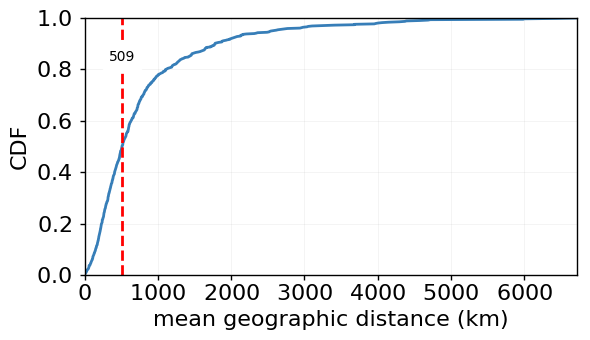
\epsfig{file=figs/geo_means.png, width=1\linewidth}
    \caption{CDF of mean geographic distance between
    cluster members. The dashed vertical line marks the median.}
    \label{geomeans}
\end{figure}

Since CNRE potentially spans many, physically distinct resources, it serves as
an \emph{aggregate} measurement, and we do not attempt to pinpoint the location
of any individual resource. Instead, we identify the effective ``center'' of
each cluster and measure the effect of a member's distance from the center.
Figure \ref{centerlocs} marks a point for the the coordinates of each cluster's
center. The disproportionately high number of centers located in Europe is
byproduct of the distribution of RIPE Atlas probes, which are most densely
concentrated in Europe where RIPE operates. 

\begin{figure*}
    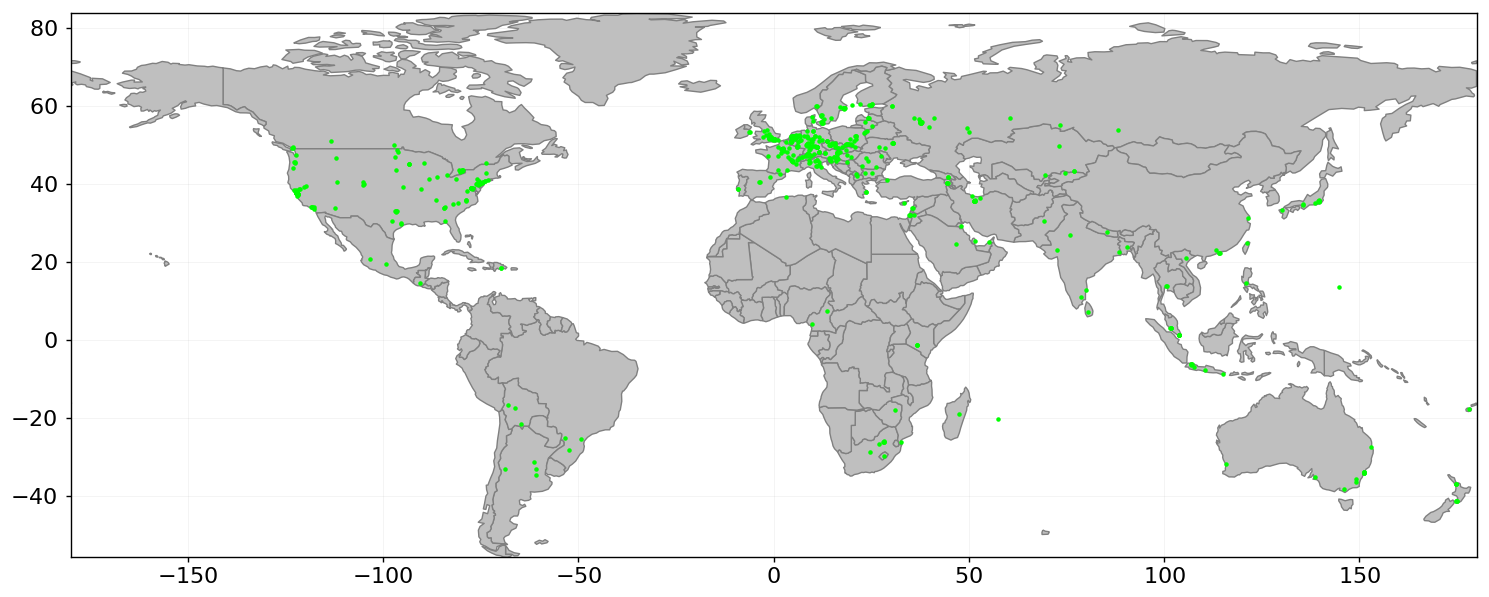
\epsfig{file=figs/geo_centers.png, width=1\linewidth}
    \caption{Map of world with point for each cluster's geographic center.}
    \label{centerlocs}
\end{figure*}


Following the intuition of DNS redirection laid out in other work
\cite{Calder2013,exploringedns,benchaita2016stability}, we hypothesize that the
geographic center of a cluster will sit physically close the location of the
most of that cluster's network resources. By this logic, clients closer to
their cluster's center should experience better network performance
(\emph{i.e.}, lower latency) than those farther away. To test this, we compared
each client's mean latency (taken across all 299 ping responsive domains in our
set) to that client's distance from its respective cluster's center. For
simplicity, we use a cluster's geometric median as an estimate of its center.
The results of this comparison are shown in Figure \ref{geoperf} as a scatter
plot of mean latency versus distance from cluster center. Each point
corresponds to a single client's latency and distance from its respective
cluster's center.  The figure also includes a best fit line, denoting the
overall trend of the points. 

Note the positive slope of points in Figure \ref{geoperf}, indicative of a
directly proportional relationship between latency and distance from the
cluster's effective center. As a client's distance from its cluster's center
increases, so does its latency. Performance for clients relatively near their
respective centers --- closer than 1000 km --- is seemingly noisy and no trend
is clearly observable.  However, as the geographic distance increases beyond
1000 km, the directly proportional relationship between performance and center
distance becomes more apparent. 

\begin{figure}
    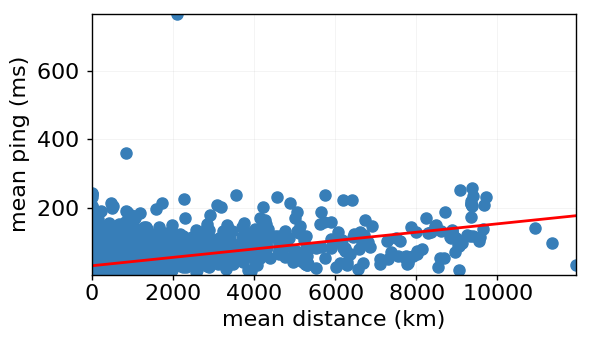
\epsfig{file=figs/geo_vs_perf.png, width=1\linewidth}
    \caption{Scatter plot where, for each client, we compare the client's mean latency
    (across all responding sites) to that client's distance from its cluster's
    center. The line denotes a first order best fit curve for the scatter plot's points.}
    \label{geoperf}
\end{figure}

Also note that the slope of Figure \ref{geoperf}'s best fit line
quantifies this relationship as approximately
$8.2\times10^{7}$m/s, which implies a general data speed of
approximately one half of the speed of light. This is comparable to the transmission speeds of the fastest network communication mediums in use at the
time of this writing --- approximately $\frac{2}{3}$rds of the speed of
light \cite{gueye2006constraint,speedoflight}. Traffic, routing complexity, and the pressence of lower speed
mediums or hops (\emph{i.e.}, bottlenecks) may account for the apparently lower speed in our finding.


\begin{figure}
        \begin{subfigure}[b]{0.8\linewidth}
            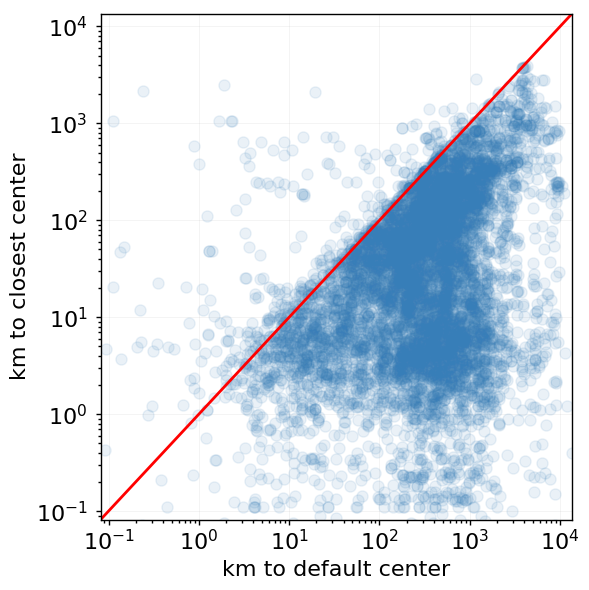
\epsfig{file=figs/nearest_centers_dist.png, width=1\linewidth}
            \caption{geographic distance}
            \label{nearest_center_dist}
        \end{subfigure}
        \begin{subfigure}[b]{0.8\linewidth}
            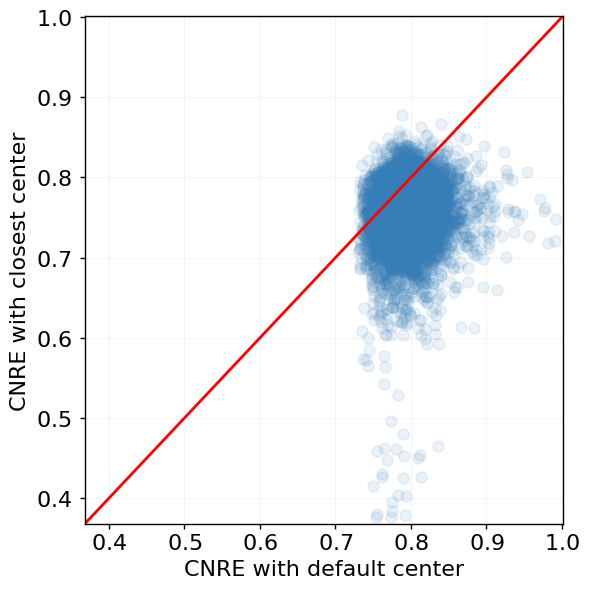
\epsfig{file=figs/nearest_centers_cnre.png, width=1\linewidth}
            \caption{CNRE similarity}
            \label{nearest_center_cnre}
        \end{subfigure}
    \caption{Subfigure \ref{nearest_center_dist} shows a scatter plot of each client's geographic distance from its own
    (``default'') cluster's
    center location versus its geographic distance to the geographically closest center of
    another cluster (``closest'').
    Subfigure \ref{nearest_center_cnre} shows a scatter plot of each client's CNRE similarity with its own
    (``default'') cluster's
    center location versus its CNRE similarity with the geographically
    closest center of
    another cluster (``closest'').}
    \label{nearest_centers}
\end{figure}

As we have demonstrated that one's distance from their cluster's center impacts
performance, clients should ideally share resources with the closest cluster
center possible. Figure \ref{geoperf} raises an additional concern: many clients
are very far away --- often thousdands of kilometers --- from their respective
cluster centers.  For perspective, we remind the reader that the circumference of
the world is approximately 40,075 km; several clients reside over a fourth of
that distance from their cluster's center. With such large geographic distances,
however, it is likely the case that there exists some \emph{alternative} cluster
whose center is geographically nearer to the client than the client's own
cluster's center. For clarity, we will refer to a client's own cluster's center
as its ``default'' center, and the cluster center geographically closest to the
client (excluding the ``default'' center) as the ``closest center'' or
``alternative center''. In Figure \ref{nearest_centers}, we compare the
properties of each client's default and closest centers.

Subfigure \ref{nearest_center_dist} shows a scatter plot of the geographic
distance from each client (in kilometers) to its default and closest centers.
The diagonal line dividing the plot indicates where the geographic distances are
equal.  Points beneath the line correspond to clients who are closer to their
alternative centers, while clients with points above the line are closest to
their default centers. Most clients are closer to their alternative centers, but
there are several details to note, discussed below. 

First, it is apparent that most clients are geograhpically closer to their
alternative cluster centers than their default centers, in some cases by orders
of magnitude. Second, we remind the reader that we employed the complete linkage
method to form our hierarchical clusters. Because of the behavior of complete
linkage, which determines cluster membership by pairwise distance across all
members instead of individual members, it is possible that individual clients
may have a higher CNRE similarity with their alternative center than with their
default center. In other words, it may be the case that we have assigned some
clients to the ``wrong'' cluster. Occurrances of this may account for some of
the noise observed in default center distances below 1000 km in Figure
\ref{geoperf}. To test for mismatched clients, we plot a point for each client's CNRE similarity
towards its closest center versus its default center in Subfigure
\ref{nearest_center_cnre}. The majority of CNRE
values in Subfigure \ref{nearest_center_cnre} are concentrated between 0.7 and
0.8. This suggests that geograhpically overlapping resource allocation groups
may be responsible for the behavior observed in the ambiguous regions of Figures
\ref{fig:dendrogram} and \ref{fig:vslabel}. 

Although 95.18\% of clients had alternative centers geographically closer than
their default centers (274.69 kilometers closer in the median case), 16.48\% of
these geographically closer 
clients had higher CNRE similarity with their default centers (1.99\% higher in
the median case). While we have demonstrated that high geographic distance
coupled with high CNRE tends to result in higher latency, here we paradoxically
observe that this arrangement is a common occurence. We further explore the
implications of this pattern in Section \ref{discussion}.

